\subsection{Openstack: a toolkit for building cloud}

\begin{itemize}

	\item Open source project.

	\item Composed of several components (nova, swift, Quantum, Glance, ...).

	\item No dynamic scheduling.

	\item Use an AMQP (Advanced Message Queuing Protocol) for inter-components communication.

\end{itemize}



\subsection{DVMS: a dynamic scheduling algorithm}

\begin{itemize}

	\item We have developed a dynamic scheduler for virtual machines.

	\item Based on a locality aware p2p overlay.

	\item Successfuly tested in simulator (simgrid) and computing grid (grid'5000).

\end{itemize}


\subsection{Integration of DVMS in Openstack}

\begin{itemize}

\item We propose to replace "nova-scheduler" (static scheduler) by DVMS.

\item Use of a "Proxy": it will be responsible for adapting "nova-scheduler" messages to DVMS and vice versa.

\begin{figure*}
	\centering
	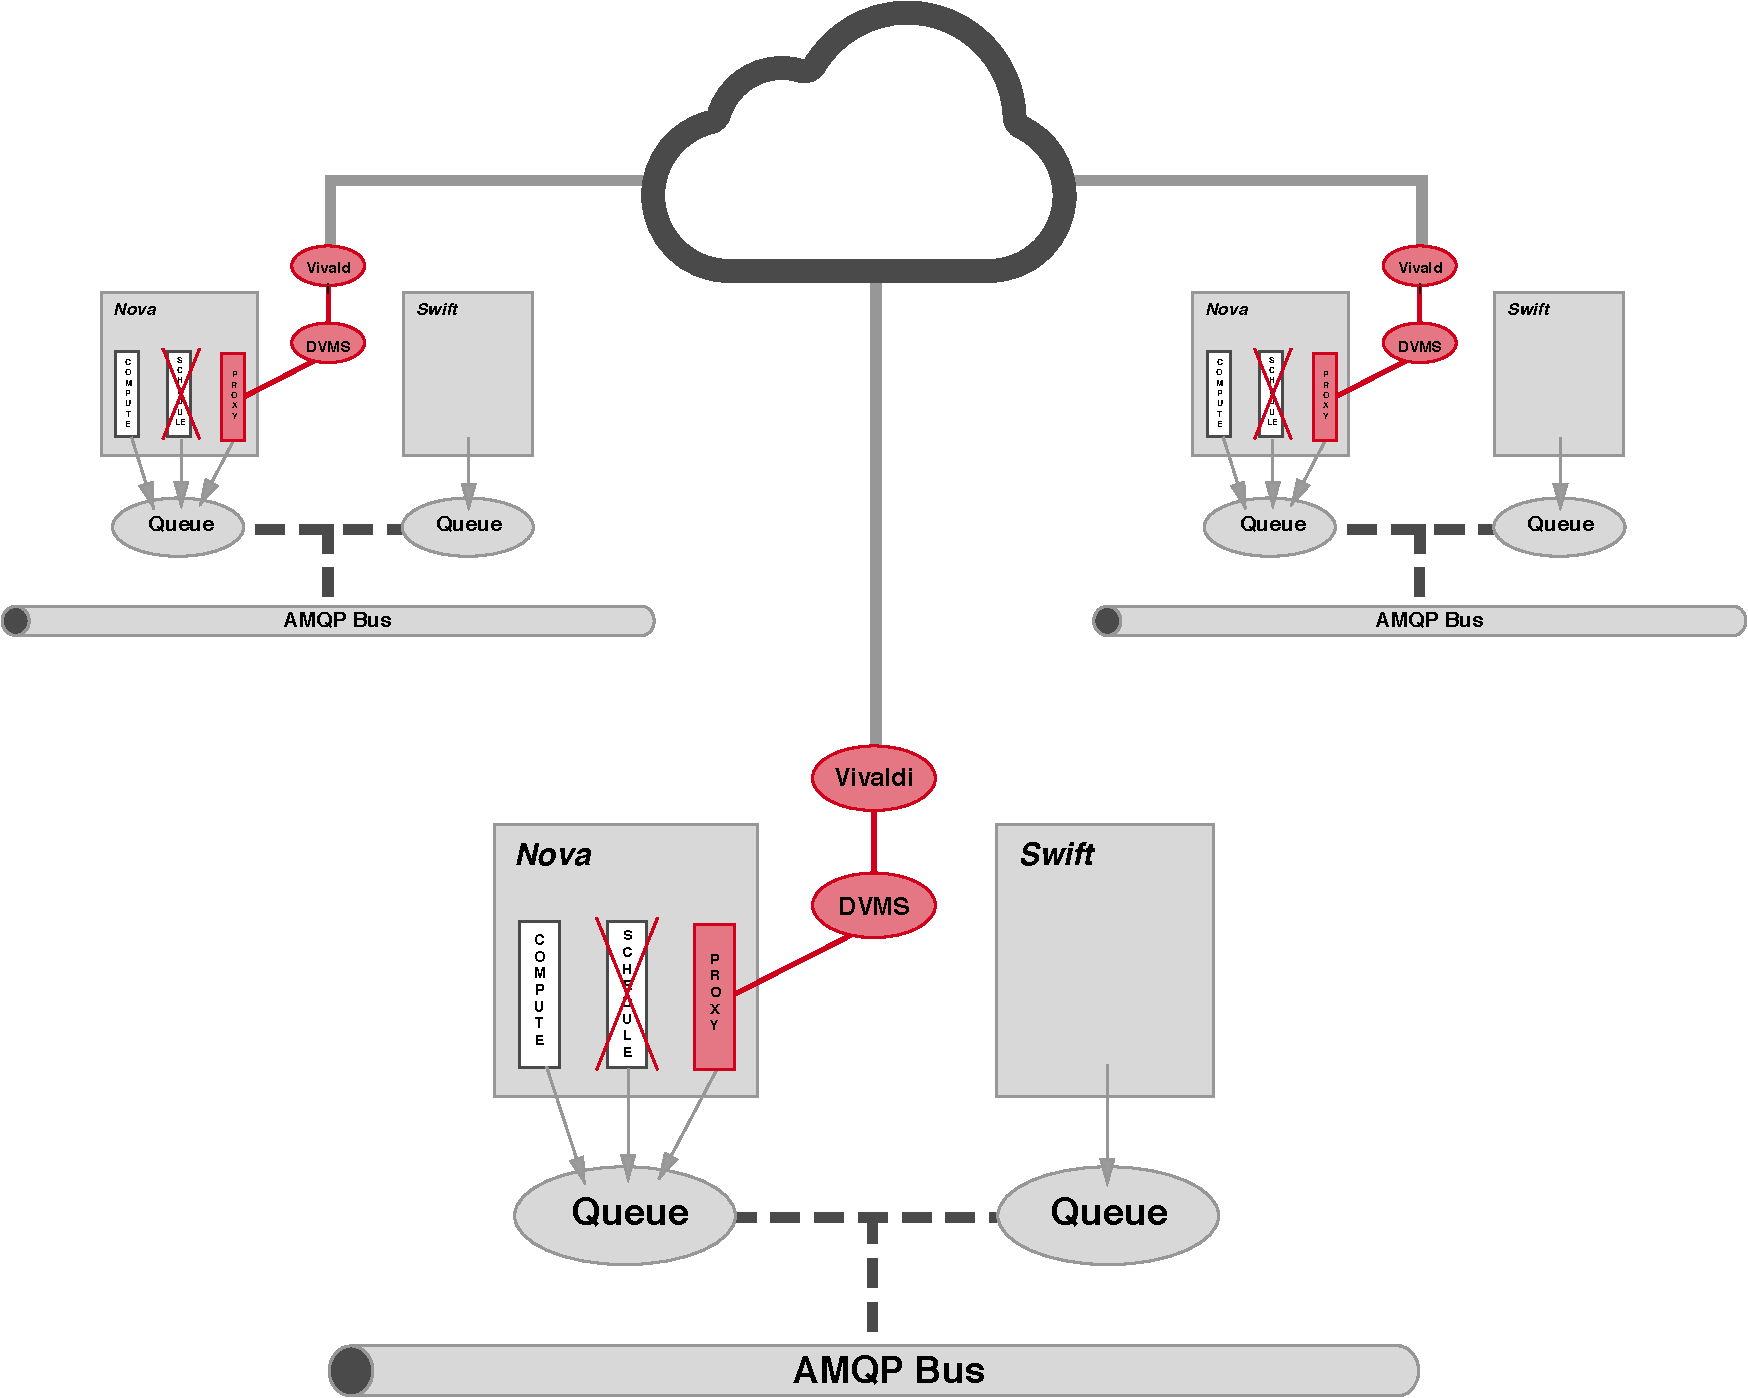
\includegraphics[width=0.75\linewidth]{Figures/openstack_dvms.pdf}
	\caption{Integration of DVMS in Openstack.}%
	\label{fig:mcd}%
	%\vspace*{-.8cm}
\end{figure*}

\end{itemize}